\nonstopmode
\documentclass{llncs}
\usepackage{graphicx}
\usepackage{verbatim}
\usepackage{amssymb}
\newcommand{\Butterfly}{\mbox{\large $\rhd\!\!\!\lhd$}}
\newcommand{\sync}[1]{\raisebox{-1.0ex}{$\;\stackrel{\Butterfly}{\scriptscriptstyle #1}\,$}}
\title{Bio-PEPA Model Report}
\author{Bio-PEPA Workbench}
\institute{\today}
\begin{document}
\maketitle
\section{Bio-PEPA model}
\begin{eqnarray*}
\mathit{contactyy} & = & [(k_1/(\mathit{Ry} + \mathit{Ry} + \mathit{Iy} + \mathit{Iy} + \mathit{Sy} + \mathit{Sy}))\times \mathit{Sy}\times \mathit{Iy}]\\%
\mathit{contactym} & = & [(k_2/(\mathit{Ry} + \mathit{Rm} + \mathit{Iy} + \mathit{Im} + \mathit{Sy} + \mathit{Sm}))\times \mathit{Sy}\times \mathit{Im}]\\%
\mathit{contactyo} & = & [(k_1/(\mathit{Ry} + \mathit{Ro} + \mathit{Iy} + \mathit{Io} + \mathit{Sy} + \mathit{So}))\times \mathit{Sy}\times \mathit{Io}]\\%
\mathit{contactmy} & = & [(k_3/(\mathit{Rm} + \mathit{Ry} + \mathit{Im} + \mathit{Iy} + \mathit{Sm} + \mathit{Sy}))\times \mathit{Sm}\times \mathit{Iy}]\\%
\mathit{contactmm} & = & [(k_4/(\mathit{Rm} + \mathit{Rm} + \mathit{Im} + \mathit{Im} + \mathit{Sm} + \mathit{Sm}))\times \mathit{Sm}\times \mathit{Im}]\\%
\mathit{contactmo} & = & [(k_5/(\mathit{Rm} + \mathit{Ro} + \mathit{Im} + \mathit{Io} + \mathit{Sm} + \mathit{So}))\times \mathit{Sm}\times \mathit{Io}]\\%
\mathit{contactoy} & = & [(\mathit{k6}/(\mathit{Ro} + \mathit{Ry} + \mathit{Io} + \mathit{Iy} + \mathit{So} + \mathit{Sy}))\times \mathit{So}\times \mathit{Iy}]\\%
\mathit{contactom} & = & [(k_2/(\mathit{Ro} + \mathit{Rm} + \mathit{Io} + \mathit{Im} + \mathit{So} + \mathit{Sm}))\times \mathit{So}\times \mathit{Im}]\\%
\mathit{contactoo} & = & [(\mathit{k7}/(\mathit{Ro} + \mathit{Ro} + \mathit{Io} + \mathit{Io} + \mathit{So} + \mathit{So}))\times \mathit{So}\times \mathit{Io}]\\%
\mathit{recoveryy} & = & [r_1\times \mathit{Iy}]\\%
\mathit{recoverym} & = & [r_2\times \mathit{Im}]\\%
\mathit{recoveryo} & = & [\mathit{r3}\times \mathit{Io}]\\%
\mathit{deathy} & = & [\mathit{r4}\times \mathit{Iy}]\\%
\mathit{deathm} & = & [\mathit{r5}\times \mathit{Im}]\\%
\mathit{deatho} & = & [\mathit{r6}\times \mathit{Io}]\\%
%
\mathit{Iy} & = & (\mathit{contactyy},1){\uparrow}\mathit{Iy} + (\mathit{contactym},1){\uparrow}\mathit{Iy} + (\mathit{contactyo},1){\uparrow}\mathit{Iy} + (\mathit{contactmy},1)\oplus  + (\mathit{contactoy},1)\oplus  + (\mathit{recoveryy},1){\downarrow}\mathit{Iy} + (\mathit{deathy},1){\downarrow}\mathit{Iy}\\%
\mathit{Im} & = & (\mathit{contactym},1)\oplus  + (\mathit{contactmy},1){\uparrow}\mathit{Im} + (\mathit{contactmm},1){\uparrow}\mathit{Im} + (\mathit{contactmo},1){\uparrow}\mathit{Im} + (\mathit{contactom},1)\oplus  + (\mathit{recoverym},1){\downarrow}\mathit{Im} + (\mathit{deathm},1){\downarrow}\mathit{Im}\\%
\mathit{Io} & = & (\mathit{contactyo},1)\oplus  + (\mathit{contactmo},1)\oplus  + (\mathit{contactoy},1){\uparrow}\mathit{Io} + (\mathit{contactom},1){\uparrow}\mathit{Io} + (\mathit{contactoo},1){\uparrow}\mathit{Io} + (\mathit{recoveryo},1){\downarrow}\mathit{Io} + (\mathit{deatho},1){\downarrow}\mathit{Io}\\%
\mathit{Sy} & = & (\mathit{contactyy},1){\downarrow}\mathit{Sy} + (\mathit{contactym},1){\downarrow}\mathit{Sy} + (\mathit{contactyo},1){\downarrow}\mathit{Sy}\\%
\mathit{Sm} & = & (\mathit{contactmy},1){\downarrow}\mathit{Sm} + (\mathit{contactmm},1){\downarrow}\mathit{Sm} + (\mathit{contactmo},1){\downarrow}\mathit{Sm}\\%
\mathit{So} & = & (\mathit{contactoy},1){\downarrow}\mathit{So} + (\mathit{contactom},1){\downarrow}\mathit{So} + (\mathit{contactoo},1){\downarrow}\mathit{So}\\%
\mathit{Ry} & = & (\mathit{recoveryy},1){\uparrow}\mathit{Ry}\\%
\mathit{Rm} & = & (\mathit{recoverym},1){\uparrow}\mathit{Rm}\\%
\mathit{Ro} & = & (\mathit{recoveryo},1){\uparrow}\mathit{Ro}\\%
D & = & (\mathit{deathy},1){\uparrow}D + (\mathit{deathm},1){\uparrow}D + (\mathit{deatho},1){\uparrow}D\\%
(\mathit{Iy} {\parallel} \mathit{Im} {\parallel} \mathit{Io} {\parallel} \mathit{Sy} {\parallel} \mathit{Sm} {\parallel} \mathit{So} {\parallel} \mathit{Ry} {\parallel} \mathit{Rm} {\parallel} \mathit{Ro} {\parallel} D)%
\end{eqnarray*}

\begin{figure}[htbp]
\begin{center}
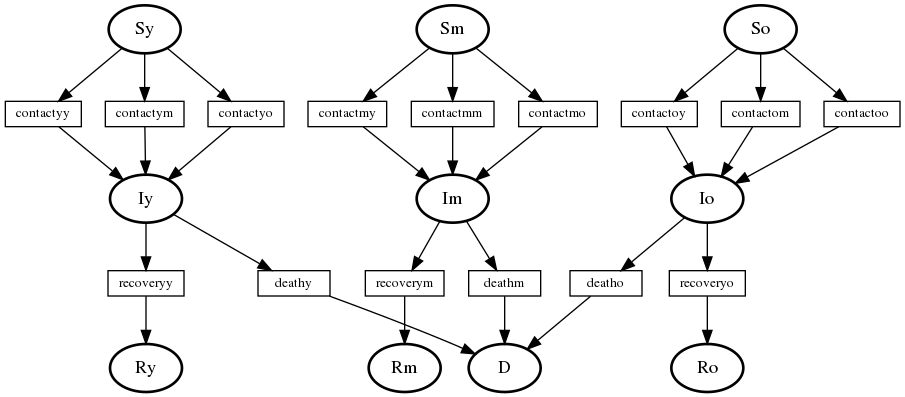
\includegraphics[width=0.6\textwidth]{dot/example_classes.pdf}
\caption{Reaction network}
\end{center}
\end{figure}
\newpage
\section{Graphs from Bio-PEPA model}
\includegraphics[scale=1]{png/example_classes001_sundials_results_0}
\appendix
\newpage
\section{Bio-PEPA input file}
\verbatiminput{example_classes.biopepa}
\newpage
\section{Dizzy equivalent input file}
\verbatiminput{dizzy/example_classes001.dizzy}
\newpage
\section{PRISM equivalent input file}
\verbatiminput{prism/example_classes001.sm}
\end{document}
